\chapter{Integration I}

In this chapter we will present an introduction to using hybrid sets for integration.
This will focus on the intuition behind it and the ``normal use case'' of integrals.
Following this, in the next chapter, we will delve more deeply from a measure theoretic perspective

\section{Single variable integration}

Given a function $f$ with real variable $x$ and an interval $[a,b]$ on the (extended) real line a traditional \textbf{definite integral} given by
\begin{equation*}
	\int_a^b f(x) \; dx
\end{equation*}
is the signed area bounded by $f$ between $x=a$ and $x=b$.
Defining the definite integral using intervals is a bit of a misnomer.
Consider the case where $a > b$ then one would typically use the identity,
\begin{equation}
	\int_a^b f(x) \; dx = - \int_b^a f(x) \; dx
\end{equation}
to evaluate the integral.
However, using the typical set builder construction ( that is, $[a,b] = \{ x | a \leq x \leq b \}$ ) it does \emph{not} follow that:
\begin{equation}
	\int_{[a,b]} f(x) \; dx = - \int_{[b,a]} f(x) \; dx
\end{equation}
since at least one interval will be empty.


\begin{definition}
Given a function $f$ with real variable $x$ and an oriented interval $I$ over $\mathbb{R}$, the integral is...
\end{definition}

If oriented intervals are used instead of traditional intervals, then the identity from xxxx \todo{Eqn number} can instead just be a result of \emph{bi-linearity}.
\begin{equation}
	\int_{[\![a,b)\!)} f(x) \; dx = - \int_{\ominus [\![a,b)\!)} f(x) \; dx = - \int_{[\![b,a)\!)} f(x) \; dx
\end{equation}


\begin{definition}
	Let $[\![ a,b ]\!]$ be an interval on $\mathbb{R}$ then the boundary function $\partial$ is the linear map such that:
	\begin{equation}
		\partial( \;[\![a,b]\!]\; ) = \hset{ a^1, b^{-1} }
	\end{equation}
\end{definition}

By linearity we also have:

$\partial (\!(a,b)\!) = \partial ( \; \ominus [\![b,a]\!] \; )= \ominus \partial ( \; [\![b,a]\!] \; ) = \ominus \hset{ b^1, a^{-1} } = \hset{ a^1, b^{-1}}$.

Using this we also have:

$\partial [\![a,b)\!) = \partial ( [\![a,c]\!] \oplus (\!(c,b)\!) ) = \partial [\![a,c]\!] \oplus \partial (\!(c,b)\!) =  \hset{ a^1, c^{-1} } \oplus \hset{ c^1, b^{-1} } = \hset{a^1, b^{-1} }$

And by a similar proof for $\partial (\!(a,c]\!]$, we conclude that:
\begin{equation}
	\partial [\![a,b]\!] = \partial [\![a,b)\!) = \partial (\!(a,b]\!] = \partial (\!(a,b)\!)
\end{equation}


Informally, isolated points do not affect the boundary of an oriented interval.
This should have been obvious from the definition to begin with.
The interval $[\![ a,a ]\!]$ is a hybrid set which contains only the element $a$ with multiplicity one.
From equation XX,
\begin{equation}
	\partial [\![ a,a ]\!] = \hset{a^1, a^{-1}} = \emptyset
\end{equation}

So whether we use $\int_a^b$ to denote the integral over the intervals $[\![a,b]\!]$, $[\![a,b)\!)$ or  $(\!(a,b)\!)$ the boundary is unchanged and so the integral will evaluate identically.

The hybrid sets $[\![a,b]\!] \oplus [\![b,c]\!]$ and $(\!(a,b)\!) \oplus (\!(b,c)\!)$ have identical multiplicities almost everywhere.
At $b$, they will differ by 2. 
Although simple arguments resolve this issue, by using left-closed, right-open oriented intervals we can bypass these arguments altogether when showing
\begin{equation}
	\int_{[\![a,b)\!)} f(x) \; dx + \int_{[\![b,c)\!)} f(x) \; dx = \int_{[\![a,c)\!)} f(x) \; dx
\end{equation}

Somewhere in this section:

- ``For now we will ignore the underlying integration mechanics and focus on the intuition of using oriented intervals. In chapter X we will return to this topic from a measure theoretic perspective to establish the Lesbegue integral.''

\section{$k$-Rectangles}

For now, we will concern ourselves only with oriented, $n$-dimensional, axis-aligned rectangles in $\mathbb{R}^n$.
In one dimension, the previously discussed oriented intervals cover most obvious shapes.
Moving to two dimensions, there are many more obvious shapes to consider but we will temporarily ignore triangles, circles and even rectangles that are tilted.
First we must introduce some notation to describe these and higher dimension rectangles. 

At the moment the only rectangles we have defined are the one-dimensional ``oriented interval''.
Hence we will also refer to this as a 1-rectangle.
We construct higher dimensional $n$ rectangles using the Cartesian product.
\begin{definition}
	Let $X = \hset{ x_1^{m_1}, ... , x_k^{m_k} }$ and $Y= \hset{ y_1^{n_1}, ... , y_\ell^{n_\ell} }$ be hybrid sets.
	We define the \textbf{Cartesian product of hybrid sets $\boldsymbol{X}$ and $\boldsymbol{Y}$}, denoted with $\times$ operator as:
	\begin{equation}
		X \times Y = \hset{ (x, y)^{m \cdot n} \; : \; x^m \in X, y^n \in Y }
	 \end{equation}
\end{definition}

If $[\![a,b]\!]$ and $[\![c,d]\!]$ are both positively oriented 1-rectangles then their Cartesian product is shown in Figure 4.1 is clearly a two dimensional rectangle or \emph{2-rectangle}. 
Taking the Cartesian product of a 2-rectangle and 1-rectangle gives a 3-rectangle in $\mathbb{R}^3$. 
We should note here that we do not distinguish between $((x,y),z)$ and $(x,(y,z))$ but rather we treat both as different names for the ordered triple $(x,y,z)$.
We similarly associate parentheses in higher dimensions as well.

\begin{figure}[h]
\caption[Cartesian product of two 1-rectangles]{The Cartesian product of two positively oriented 1-rectangles $[\![a,b]\!]$ and $[\![c,d]\!]$ is a positively oriented 2-rectangle.}
\centering
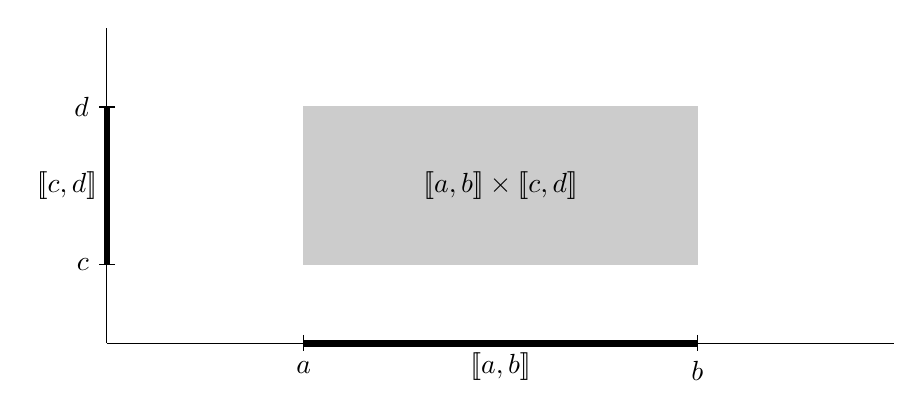
\begin{tikzpicture}[y=1cm, x=2.5cm]	
 	%axis
	\draw(0,0) -- coordinate (x axis mid) (4,0);
    	\draw (0,0) -- coordinate (y axis mid) (0,4);
    	
    	%ticks
    	\draw[fill] (1,1pt) rectangle (3,-1pt);    	
    	\draw (1, 3pt) -- (1, -3pt) node[anchor=north] {$a$};
    	\draw (3, 3pt) -- (3, -3pt) node[anchor=north] {$b$};
    	\draw (2, 0) node[anchor=north] {$[\![a,b]\!]$};
    	
    	\draw[fill] (1pt,1) rectangle (-1pt, 3);
    	\draw (3pt, 1) -- (-3pt, 1) node[anchor=east] {$c$};
    	\draw (3pt, 3) -- (-3pt, 3) node[anchor=east] {$d$};
    	\draw (0,2) node[anchor=east] {$[\![c,d]\!]$};
    	
    	\draw[fill, color=black!20] (1,1) rectangle (3,3);
    	\draw (2, 2) node {$[\![a,b]\!] \times [\![c,d]\!]$ };
\end{tikzpicture}
\end{figure}

\begin{theorem}
	The Cartesian product of a $k$-rectangle in $\mathbb{R}^m$ (where, $k\leq m$) 
	and $\ell$-rectangle in $\mathbb{R}^n$ (again, $\ell \leq n$) 
	is a $(k+\ell)$-rectangle in $\mathbb{R}^{m+n}$.
\end{theorem}

For completeness we will also define a 0-rectangle as a hybrid set containing a single point with multiplicity $1$ or $-1$.
Firstly this allows us to embed $k$-rectangles in $\mathbb{R}^n$.
For example $[\![a,b]\!] \times [\![c,d]\!] \times \hset{e^1}$ is the product of two 1-rectangles and a 0-rectangle (all over $\mathbb{R}$) and so it is a 2-rectangle over $\mathbb{R}^3$.
Specifically, it is the 2-rectangle $[\![a,b]\!] \times [\![c,d]\!]$ on the plane $z=3$.
This also illustrates the principle that given a $k$-rectangle in $\mathbb{R}^n$ where $n>k$ we can always find a $k$ dimensional subspace which also contains the rectangle.

\todo{segue into notation}

\begin{definition}
	Let $\boldsymbol{a} = (a_1, a_2, \ldots, a_n)$ and 
	$\boldsymbol{b} = (b_1, b_2, \ldots, b_n)$ be ordered $n$-tuples then we define:
	\begin{equation*}
		[\![ \boldsymbol{a}, \boldsymbol{b} ]\!] 
		= [\![a_1, b_1]\!] \times [\![a_2, b_2 ]\!] \times \ldots \times [\![a_n , b_n]\!]
	\end{equation*}
\end{definition}

The dimension of $[\![ \boldsymbol{a}, \boldsymbol{b} ]\!]$ is equal to the number of indices where $a_i$ and $b_i$ are distinct.
For any $i$ where $a_i = b_i$, the resulting term: $[\![ a_i, b_i ]\!]$ will be a 0-rectangle and will not increase the overall dimension.
Comparatively, the orientation of $[\![ \boldsymbol{a}, \boldsymbol{b} ]\!]$ is based on the number of negatively oriented intervals in its terms.
Should there be an odd number of indices $i$ such that $a_i > b_i$ then $[\![ \boldsymbol{a}, \boldsymbol{b} ]\!]$ will also be negatively oriented.
Otherwise, it will be positively oriented. 


In one dimension, the boundary of an interval was quite straight-forward.
For a positively oriented interval, the boundary was composed of two points; 
the right end-point was positive and the left end-point was negative.
From the perspective of $k$-rectangles, 
the $\partial$ operator has mapped an oriented 1-rectangle to a set of oriented 0-rectangles.
We will now generalize the boundary to map an oriented $n$-rectangle to an $(n-1)$-rectangle.

\begin{definition}
	Let $\boldsymbol{a} = (a_1, \ldots, a_n)$ and $\boldsymbol{b} = (b_1, \ldots, b_n)$ be $n$-tuples over $\mathbb{R}$ as defined earlier. 
	The \textbf{boundary of $ \boldsymbol{[\![ a,b ]\!]} $ }, denoted the operator $\partial$ is given by
	\begin{equation*}
		\partial \left( [\![ \boldsymbol{a}, \boldsymbol{b} ]\!] \right) 
		= \bigoplus_{i=1}^n (-1)^i 
			\left(	
			[\![\boldsymbol{a}^{[\![1,i)\!)}, \boldsymbol{b}^{[\![1,i)\!)} ]\!]
			\times a_i \times
			[\![\boldsymbol{a}^{(\!(i,n]\!]}, \boldsymbol{b}^{(\!(i,n]\!]} ]\!]
			\ominus
			[\![\boldsymbol{a}^{[\![1,i)\!)}, \boldsymbol{b}^{[\![1,i)\!)} ]\!]
			\times b_i \times
			[\![\boldsymbol{a}^{(\!(i,n]\!]}, \boldsymbol{b}^{(\!(i,n]\!]} ]\!]
			\right)
	\end{equation*}
\end{definition}

The above equation will require a bit of unpacking to digest.
Two different types of oriented intervals appear.
The first appears as superscripts to $\boldsymbol{a}$ and $\boldsymbol{b}$ and is an interval over vector indices just as in Chapter 3.
Thus, the term $\boldsymbol{a}^{[\![1,i)\!)}$ refers to the vector $(a_1, a_2, \ldots, a_{i-1})$ 
while the term $\boldsymbol{b}^{(\!(i,n]\!]}$ refers to $(b_{i+1}, b_{i+2}, \ldots, b_{n})$.
This provides a compact notation to partition the original range of indices into 3 pieces: $[\![ 1,i )\!)$, $[\![i, i]\!]$, and $(\!(i, n]\!]$.
The first and last portions are isolated but left untouched, 
but the central $[\![i,i]\!]$ term is then replaced with the 0-rectangles $a_i$ or $b_i$.
Formally, we are actually using the hybrid sets $\hset{(a_i)^1}$ and $\hset{(b_i)^1}$ but we write $a_i$ and $b_i$ for clarity.

Each Cartesian product forms a $(k-1)$-rectangular face of the $k$-rectangle which we shall show.
Let $[\![ \boldsymbol{a}, \boldsymbol{b} ]\!]$ be a $k$ rectangle in $\mathbb{R}^n$.
Following from definitions we have:
\begin{equation}
	[\![ \boldsymbol{a}, \boldsymbol{b} ]\!] = 
		[\![\boldsymbol{a}^{[\![1,i)\!)}, \boldsymbol{b}^{[\![1,i)\!)} ]\!] \times 
		[\![\boldsymbol{a}^{[\![i,i]\!]}, \boldsymbol{b}^{[\![i,i]\!]} ]\!] \times
		[\![\boldsymbol{a}^{(\!(i,n]\!]}, \boldsymbol{b}^{(\!(i,n]\!]} ]\!]
\end{equation}
If $a_i$ and $b_i$ are distinct then $[\![\boldsymbol{a}^{[\![i,i]\!]}, \boldsymbol{b}^{[\![i,i]\!]} ]\!]$ is a 1-rectangle.
Since both $a_i$ and $b_i$ are 0-rectangles and expressions agree everywhere else, then the following are both $(k-1)$-rectangles:
\begin{align}
	[\![\boldsymbol{a}^{[\![1,i)\!)}, \boldsymbol{b}^{[\![1,i)\!)} ]\!]
	\times a_i \times
	[\![\boldsymbol{a}^{(\!(i,n]\!]}, \boldsymbol{b}^{(\!(i,n]\!]} ]\!]
	\\
	[\![\boldsymbol{a}^{[\![1,i)\!)}, \boldsymbol{b}^{[\![1,i)\!)} ]\!]
	\times b_i \times
	[\![\boldsymbol{a}^{(\!(i,n]\!]}, \boldsymbol{b}^{(\!(i,n]\!]} ]\!]
\end{align}
However if $a_i = b_i$ then $[\![\boldsymbol{a}^{[\![i,i]\!]}, \boldsymbol{b}^{[\![i,i]\!]} ]\!]$ is a 0-rectangle and so the expressions in (4.10) and (4.11) are both $k$-rectangles!
Since $a_i = b_i$, the two expressions are identical, so their difference is zero and the terms disappear.

\subsection{Example: \emph{Boundary of a 1-rectangle}}

Let $\boldsymbol{a}= (a_1)$ and $\boldsymbol{b} = (b_1)$ be trivial 1-tuples. 
It follows that:
\begin{align*}
	\partial ( \; [\![ \boldsymbol{a}, \boldsymbol{b} ]\!] \; )
	=& \; (-1)^i ( [\![\boldsymbol{a}^{[\![1,1)\!)}, \boldsymbol{b}^{[\![1,1)\!)} ]\!]
	\times a_1 \times
	[\![\boldsymbol{a}^{(\!(1,1]\!]}, \boldsymbol{b}^{(\!(1,1]\!]} ]\!]\\
	&\; \ominus
	[\![\boldsymbol{a}^{[\![1,1)\!)}, \boldsymbol{b}^{[\![1,1)\!)} ]\!]
	\times b_1 \times
	[\![\boldsymbol{a}^{(\!(1,1]\!]}, \boldsymbol{b}^{(\!(1,1]\!]} ]\!] )\\
	=& \; \ominus [\![\boldsymbol{a}^{\emptyset}, \boldsymbol{b}^{\emptyset} ]\!]
	\times a_1 \times
	[\![\boldsymbol{a}^{\emptyset}, \boldsymbol{b}^{\emptyset} ]\!]\\
	& \; \oplus
	[\![\boldsymbol{a}^{\emptyset}, \boldsymbol{b}^{\emptyset} ]\!]
	\times b_1 \times
	[\![\boldsymbol{a}^{\emptyset}, \boldsymbol{b}^{\emptyset} ]\!] \\
	=& \; b_1 \ominus a_1
\end{align*}
Again, we omit the braces from the hybrid sets $\hset{(a_1)^1}$ and $\hset{(b_1)^1}$.
Recalling from the previous section in (4.4), we can see that the results agree:
\begin{equation}
	\partial ( \; [\![ a_1 ,b_1 ]\!] \; ) = b_1 \ominus a_1 = \hset{(b_1)^1} \ominus \hset{(a_1)^1} = \hset{(a_1)^{-1}, (b_1)^1}
\end{equation}

\subsection{Example: \emph{Boundary of a 3-rectangle}}
Let $\boldsymbol{a} = (0,0,0)$ and $\boldsymbol{b} = (1,1,1)$.
Then, the 3-rectangle formed by $[\![a,b]\!]$ in Figure 4.2.
\begin{align*}
	\partial ( \; [\![ \boldsymbol{a} , \boldsymbol{b} ]\!] \; )
	=& \; (-1)^1  \; \left( \{ 0 \} \times [\![a^{(\!(1,3]\!]},b^{(\!(1,3]\!]}]\!] \; \ominus \; \{ 1 \} \times [\![a^{(\!(1,3]\!]},b^{(\!(1,3]\!]}]\!] \right)\\
	  & \; \oplus (-1)^2 \left( [\![a^{[\![1,2)\!)}, b^{[\![1,2)\!)} ]\!] \times \{ 0 \} \times [\![a^{(\!(2,3]\!]},b^{(\!(2,3]\!]}]\!] \; \ominus \; [\![a^{[\![1,2)\!)}, b^{[\![1,2)\!)} ]\!] \times \{ 1 \} \times [\![a^{(\!(2,3]\!]},b^{(\!(2,3]\!]}]\!] \right)\\
	  & \; \oplus (-1)^3 \left( [\![0,1]\!] \times [\![0,1]\!] \times \hset{0^1} \ominus [\![0,1]\!] \times [\![0,1]\!] \times \hset{1^1} \right)
\end{align*}

\begin{figure}[h]
\caption[Unit cube with boundary]{The unit cube given as the 3-rectangle: $[\![(0,0,0), (1,1,1) ]\!]$ and the 6 faces in its boundary. }
\centering
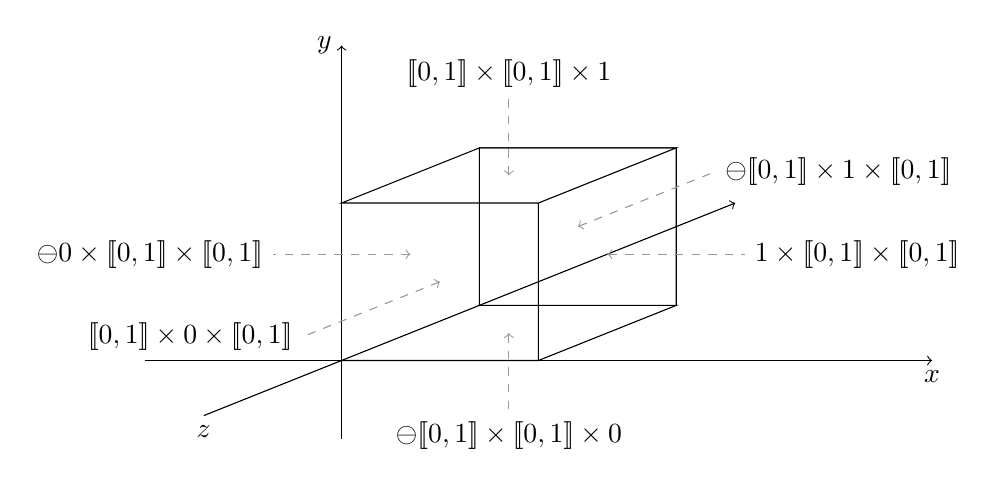
\begin{tikzpicture}[y=1cm, x=2.5cm]	
 	%axis
	\draw[->] (-1,0) -- coordinate (x axis mid) (3,0) node[anchor=north] {$x$};
    	\draw[->] (0,-1) -- coordinate (y axis mid) (0,4) node[anchor=east] {$y$};
	\draw[->] (-0.7,-0.7) node[anchor=north] {$z$} --++ (2.7,2.7) ;
	
	\draw (0,0) --++ (1,0) --++ (0,2) --++ (-1,0) --++ (0.7, 0.7) --++ (1,0) --++ (-0.7,-0.7);
	\draw (1,0) --++ (0.7, 0.7) --++ (-1,0) --++ (0,2) --++ (1,0) --++ (0,-2);
	
	\draw[color=black!40, dashed, <-] (0.35, 1.35) --++ (-0.7, 0) node[anchor=east, black] {$\ominus \hset{0} \times [\![0,1]\!] \times [\![0,1]\!]$};
	\draw[color=black!40, dashed, <-] (1.35, 1.35) --++ (0.7, 0) node[anchor=west, black] {$\hset{1} \times [\![0,1]\!] \times [\![0,1]\!]$};
	\draw[color=black!40, dashed, <-] (0.5,1) --++ (-0.7,-0.7) node[anchor=east, black] {$ [\![0,1]\!] \times \hset{0} \times [\![0,1]\!]$};
	\draw[color=black!40, dashed, <-] (1.2,1.7) --++ (0.7,0.7) node[anchor=west, black] {$\ominus [\![0,1]\!] \times \hset{1} \times [\![0,1]\!]$};
	\draw[color=black!40, dashed, <-] (0.85,0.35) --++ (0,-1) node[anchor=north, black] {$\ominus [\![0,1]\!] \times [\![0,1]\!] \times \hset{0}$};
	\draw[color=black!40, dashed, <-] (0.85,2.35) --++ (0,1) node[anchor=south, black] {$[\![0,1]\!] \times [\![0,1]\!] \times \hset{1}$};
	
\end{tikzpicture}
\end{figure}
\todo[inline]{finish diagram}

Several ways to interpret and visualize the sign.


In particular many conventions exist for the orientation of 2-rectangles in $\mathbb{R}^3$.

 - CW/CCW (interpreting the 1-rectangles in its boundary as arrows)
 
 - which induces a normal
 
 - normal can be used to backface cull as is typical in graphics 

\begin{figure}[h]
\caption[Orientations of 2-rectangles]{asdfasdfasdf }
\centering
\begin{tikzpicture}

	\def\rectCycle#1#2#3#4{
		\draw[->] (#1,#2) -- (#3,#2);
		\draw[->] (#3,#2) -- (#3,#4);
		\draw[->] (#3, #4) -- (#1,#4);
		\draw[->] (#1,#4) -- (#1,#2);
		\draw[very thick, ->] (#1, 0) -- (#3, 0);
		%\draw[fill] (#1,#2) circle (1 pt);
	}

	
	\rectCycle {0+1}{1} {0+2}{2};
	\draw[<->] (0,3) -- (0,0) -- (3,0);
	\draw[very thick, ->] (0,1) -- (0,2);
	\draw (0,1.5) node[anchor=east] {$+$};
	\draw (1.5,0) node[anchor=north] {$+$};
	\draw (1.5, 1.5) node {$+$};
	
	  
	\rectCycle {4+2}{1} {4+1}{2};
	\draw[<->] (4+0,3) -- (4+0,0) -- (4+3,0);
	\draw[very thick, ->] (4+0,1) -- (4+0,2);
	\draw (4+0,1.5) node[anchor=east] {$+$};
	\draw (4+1.5,0) node[anchor=north] {$-$};
	\draw (4+1.5, 1.5) node {$-$};
	
	
	\rectCycle {8+2}{2} {8+1}{1};
	\draw[<->] (8+0,3) -- (8+0,0) -- (8+3,0);
	\draw[very thick, ->] (8+0,2) -- (8+0,1);
	\draw (8+0,1.5) node[anchor=east] {$-$};
	\draw (8+1.5,0) node[anchor=north] {$-$};
	\draw (8+1.5, 1.5) node {$+$};
	
	
	\rectCycle {12+1}{2} {12+2}{1};
	\draw[<->] (12+0,3) -- (12+0,0) -- (12+3,0);
	\draw[very thick, ->] (12+0,2) -- (12+0,1);
	\draw (12+0,1.5) node[anchor=east] {$-$};
	\draw (12+1.5,0) node[anchor=north] {$+$};
	\draw (12+1.5, 1.5) node {$-$};
	
\end{tikzpicture}
\end{figure}


\section{Chains}

$k$-chain $C_k$ Abelian group of $k$-intervals

$\partial_k : C_k \to C_{k-1}$


\subsection{Example: \emph{Boundary of a boundary}}

Boundary of result from 4.2.2

$\partial \partial = 0$


\section{Integrating Rectangles}



\section{Integration by pull-back}

(move to Integration II?)
